\documentclass[11pt]{article}
\renewcommand{\baselinestretch}{1.05}

\usepackage{amsmath,amsthm,verbatim,amssymb,amsfonts,amscd, graphicx}
\usepackage{graphics}

\usepackage{xcolor}

\usepackage[hidelinks]{hyperref}

\usepackage{parskip}

\renewcommand{\contentsname}{Table des mati\`eres}

\topmargin0.0cm
\headheight0.0cm
\headsep0.0cm
\oddsidemargin0.0cm
\textheight23.0cm
\textwidth16.5cm
\footskip1.0cm

\begin{document}

\title{\textbf{TP Caract\'erisation} }
\author{Lucien Dos Santos \\ Mohamed Hage Hassan}
\date{21 Mars, 2017}
\maketitle

\tableofcontents
\clearpage

\section{Introduction}

Le but principal de ce TP est de caract\'eriser les 2 composantes principales du transistor MOS :

\begin{figure}[!htb]
\centering
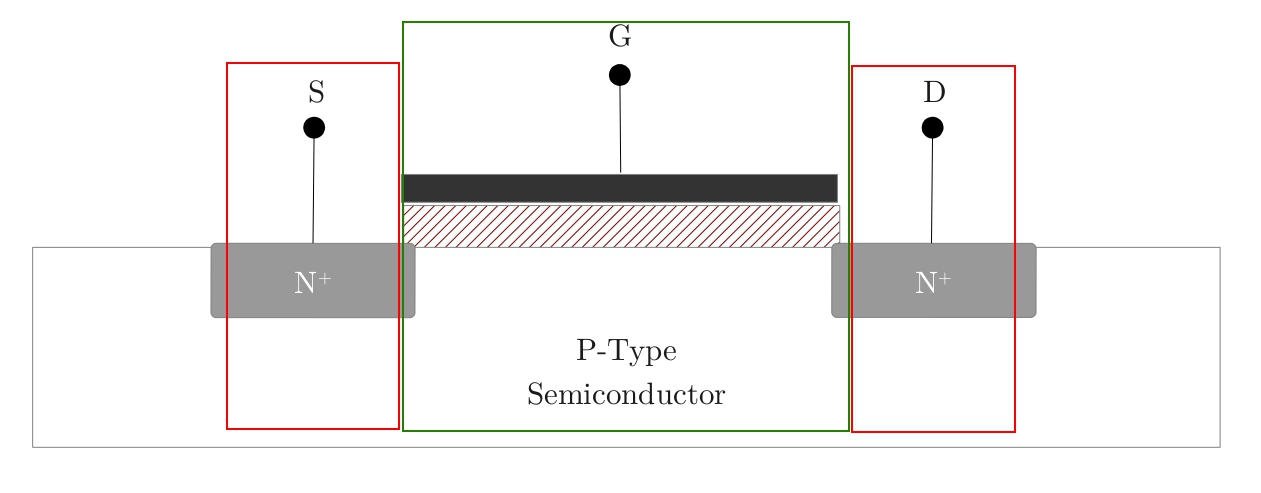
\includegraphics[scale=0.30]{mosfet_structure_implemented_side_view.jpg}
\caption{Composition du MOSFET}
\end{figure}

La capacit\'e MOS (vert) et les 2 jonctions PN (rouge) r\'esultantes des manipulations effectu\'ees en salle blanche.
On sp\'ecifie que ces 2 parties peut-\^etre utilis\'ees comme des composantes seules :

\begin{itemize}
\item \textbf{Jonction PN}

\begin{itemize}
\item[-] Capteurs thermiques (au lieu des couples thermiques).
\item[-] Capteurs optiques : photod\'eteteurs.
\item[-] Transmissions haute-fr\'equence (diode optiques).
\end{itemize}

\item \textbf{Capacit\'ees MOS}
\begin{itemize}
\item[-] Matrice de capacit\'ees MOS utilis\'ees pour la reconstruction d'une image dans les appareils photo r\'ecentes.
\end{itemize}

\end{itemize}

On note que pour la partie salle blanche, on a r\'ealiser la jonction PN :

\textbf{\'Etapes de r\'ealisation}
\begin{itemize}
\item[-] Nettoyage du wafer.
\item[-] D\'epot du $SiO_2$.
\item[-] Diffusion thermique pour le dopage du wafer (en type $n+$).
\item[-] Deposition d'une couche d'Aluminium
\item[-] Gravure d'aluminium.
\end{itemize}

\section{Caract\'erisation de la jonction PN}
On cherche \`a d\'eterminer la caract\'eristique I/V de la jonction.
L'allure g\'en\'erale du courant d'une diode en fonction de la tension est r\'epr\'esent\'ee par le sch\'ema suivant :

\begin{figure}[!htb]
\centering
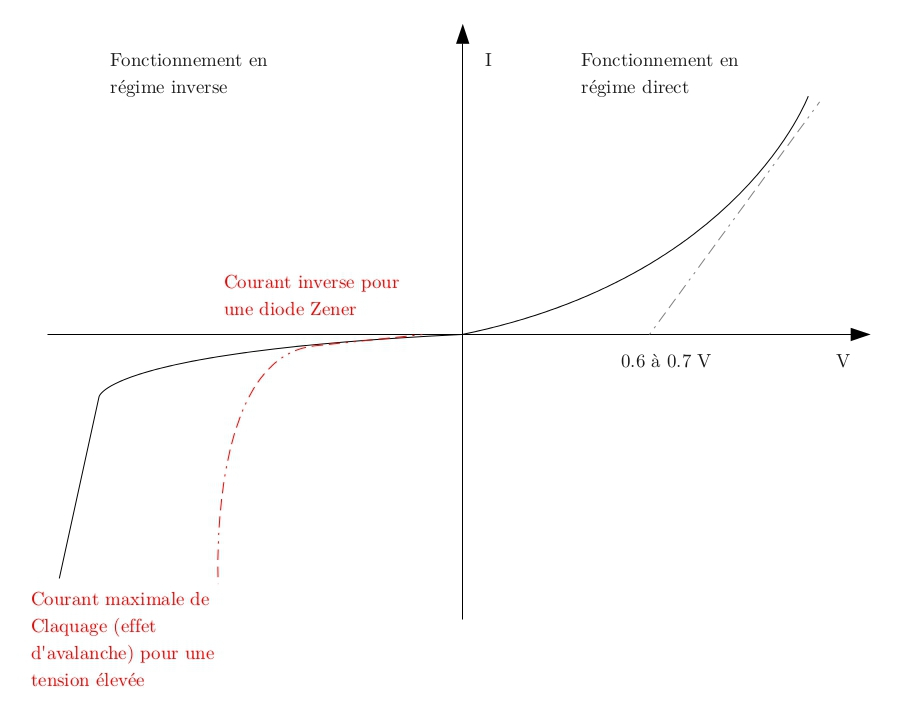
\includegraphics[scale=0.54]{carac_I_V.jpg}
\caption{R\'egime du foncitonnement de la jonction PN}
\end{figure}

On souhaite donc chercher les param\`etres : 
\begin{itemize}
\item[-] $I_S$ courant de saturation
\item[-] $V_{th}$ Tension de seuil (Thershold volatage)
\item[-] $V_a$  Tension d'avalanche
\item[-] $n$ facteur d'id\'ealit\'e
\end{itemize}
\clearpage

\subsection{M\'ethodes de d\'etermination des param\`etres}

\textbf{Courant de saturation $I_S$ et du facteur n}

Sachant que le mod\`ele math\'ematique de la diode s'exprime par :
\[
	I = I_S (e^{\frac{q V}{n K_B T}} - 1 )
\]

On constate que c'est difficile de d\'eterminer la valeur de $I_{S}$ directement, sachant qu'entre 0 et 0.6V, en zone directe de fonctionnnement, on a un ph\'enom\`ene de recombinaison des porteurs (charge d'espace). Ce phenom\`ene pr\'eexiste toujours en r\'egime inverse.

Pour se faire, on prend le mod\`ele simplifi\'e de $I$ \textbf{pour la zone directe}:

\[
	I = I_S (e^{\frac{q V}{n K_B T}})
\]
\[
\implies	ln(I) = ln(I_S) +  \frac{q V}{n K_B T}
\]

On retrouve que c'est possible de d\'eterminer ces 2 facteurs :

\begin{figure}[!htb]
\centering
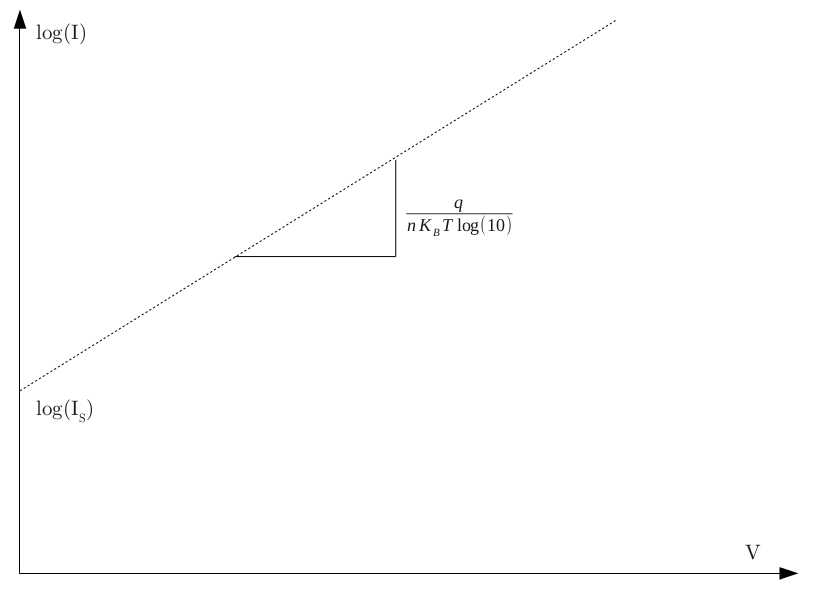
\includegraphics[scale=0.54]{log_echelle.jpg}
\caption{Passage en \'echelle logarithmique}
\end{figure}


\textbf{D\'etermination de $V_a$ et $V_{th}$} 

$V_{th}$ constitue l'intersection de l'asymptote \`a l'exponentielle de la courbe $I_{S}$ avec l'axe $ox$, et $V_{a}$ la tension pour laquelle on a une tr\`es forte d\'erive en intensit\'e.

\subsection{Partie pratique}
Pour la caract\'erisation des diodes, on utilise le Hwelett Packard 4155A Semiconductor Parameter Analyser. On vient manipuler des pointes en carbure de tungest\`ene pour la mesure des param\`etres d'une jonction PN :

\begin{figure}[!htb]
\centering
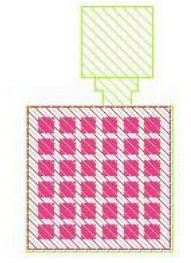
\includegraphics[scale=0.54]{diode_junction.jpg}
\caption{Diode de grande surface et petit p\'erim\`etre, surface $200 \times 200 \mu m^{2}$}
\end{figure}

La plaque principale de l'outil de mesure est polaris\'ee en inverse : on affiche les valeurs de I en fonction de V (courbe initialement \`a l'inverse), et on retrouve $V_{th} = 0.678 \phantom{2} V$.

La d\'etermination de $V_a$ s'effectue d'une fa\c con similaire : On adjuste la tension pour un balayage entre 0 et 30 V (polarization inverse) : On retrouve qu'il y a des fortes d\'erives de courant autour de 19 V. L'appareil est limit\'e en courant maximal d\'elivr\'e sur la diode, ce qui permet de protoger le wafer en cas de forte tensions.

\textbf{Calcul de n }
D'apr\`es les mesures de la pente en fonctionnement directe de la diode, on peut remonter vers le coefficient N (facteur d'id\'ealit\'e) : n = 1.76  

\section{Capaci\'e MOS}
\subsection{M\'ethodes de Calcul}
Pour caract\'eriser la capacit\'e MOS, on doit la polariser en $ V_G > V_t > 0 $ avec $V_D > 0$. Celle-ci va fonctionner en r\'egime d'inversion, la dynamique de $C=f(V)$ repr\'esente ce fonctionnement.

\clearpage

\begin{figure}[!htb]
\centering
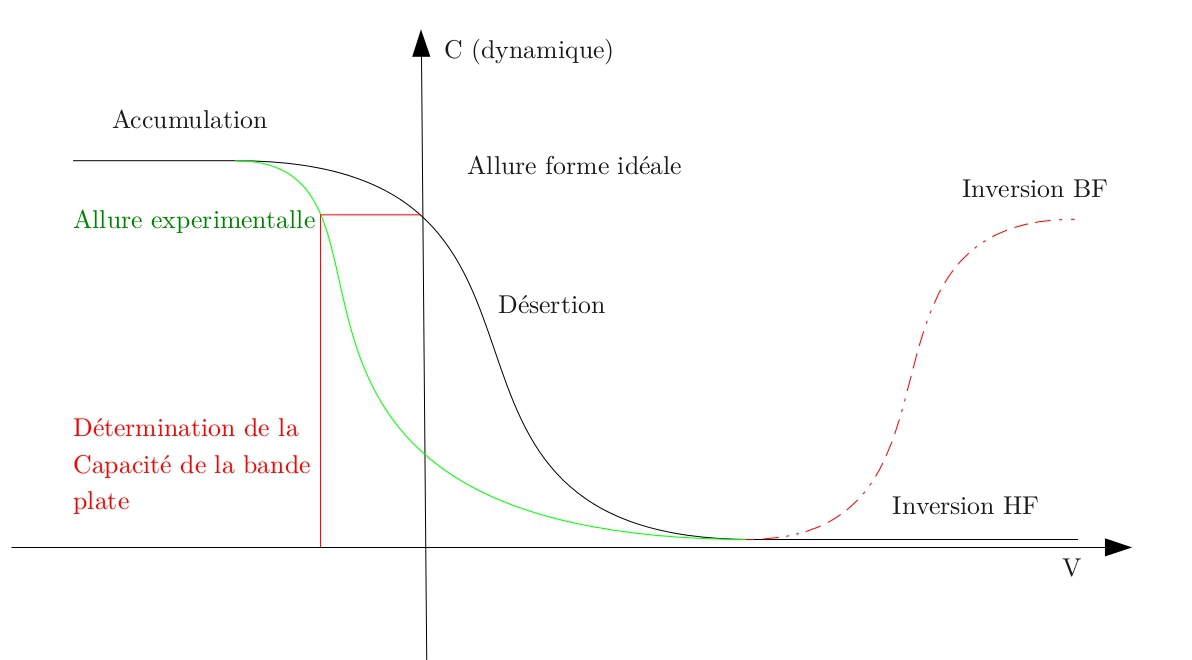
\includegraphics[scale=0.40]{allure_dynamique_MOS.jpg}
\caption{Allure de la capacit\'e MOS pour des variations de V}
\end{figure}

Le plateau form\'e par la prolongation de la zone d'accumulation d\'etermine $C_{ox} = \frac{\epsilon_{ox}}{t_{ox}}$. On peut aussi d\'eterminer la tension 
$V_{FB}$ :

\[
	V_{FB} = \Phi_{ms} - \frac{Q_{ox}}{C_{ox}}
\]

Les valeurs de $V_{FB}$, $\Phi_{ms}$ et $C_{ox}$ peuvent \^etre d\'eterminer automatiquement.

\subsection{Mise en pratique}
On v\'erfie le placement correcte du wafer dans la zone sp\'ecifi\'ee. La capacit\'ee \`a d\'eterminer est de surface $ 320 \times 200 \mu m^{2}$, et on sp\'ecifie la ``Gate work function'' pour l'Aluminium de 4.2.

On retrouve que (pour une temp\'erature de 23 C)
\begin{itemize}
\item[-] $C_{ox} = 43.5 pF$
\item[-] $R_s = 558 \Omega$
\item[-] $T_{ox} = 501 A$
\item[-] $\frac{C_{FB}}{C_{ox}} = 0.82$
\item[-] $V_{FB} = -4.57 V$
\item[-] $\Phi_{ms} = -0.869 V$
\item[-] $N_{sub} = 1.47 \times 10 ^{16} /cm^{3}$
\end{itemize}

\clearpage

Le r\'esultat de la mesure est repr\'esent\'e par la figure 6.

\begin{figure}[!htb]
\centering
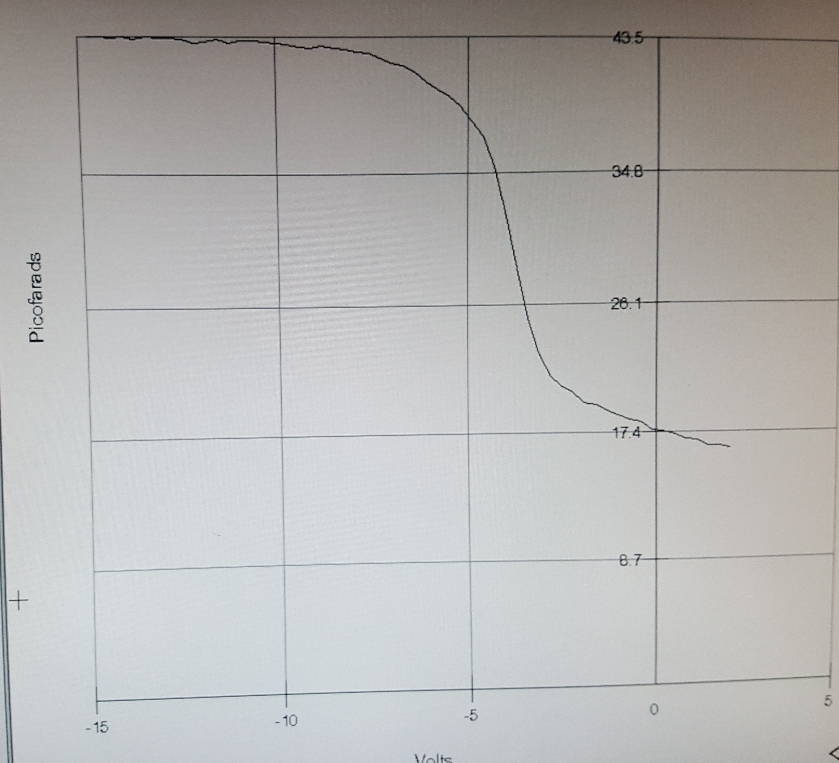
\includegraphics[scale=0.35]{allure_reelle_.jpg}
\caption{Mesure de la capacit\'e MOS pour des variations de V}
\end{figure}

On sait que : 
\[
	V_{FB} = \Phi_{ms} - \frac{Q_{ox}}{C_{ox}}
\]
\[
\implies	V_{FB} = \Phi_{ms} - \frac{Q_{ox}}{C_{ox}}
\]

\section{Conclusion}




\end{document}